\documentclass[12pt]{amsart}

%\usepackage{upgreek}
\usepackage[margin=3.5 cm]{geometry}
\usepackage{graphicx, mathabx}
\usepackage{color}
\usepackage{float}
%\usepackage{subfigure}
\newtheorem{theorem}{Theorem}[section]
\newtheorem*{theorem*}{Theorem}          %theorem without number
\newtheorem{prop}{Proposition}[section]
\newtheorem*{prop*}{Proposition}  % proposition without number
\newtheorem{coro}{Corollary}[section]
\newtheorem{lemma}[theorem]{Lemma}
\newtheorem{conj}{Conjecture}[section]
\newtheorem{obs}{Observation}[section]

\theoremstyle{definition}
\newtheorem{definition}[theorem]{Definition}
\newtheorem{example}[theorem]{Example}
\newtheorem{xca}[theorem]{Exercise}

\theoremstyle{remark}
\newtheorem{remark}[theorem]{Remark}

%\numberwithin{equation}

%    Absolute value notation
\newcommand{\abs}[1]{\left\lvert#1\right\rvert}
\newcommand{\norm}[1]{\lVert#1\rVert}
\DeclareMathOperator{\re}{Re}
\DeclareMathOperator{\im}{Im}
\newcommand{\ud}{\mathrm{d}}

\begin{document}

\title[Math 357 - Harmonic Analysis]{Isaac Viviano - Problem set no. 1}

\begin{titlepage}
  \maketitle
\end{titlepage}

\newpage \ \newpage
\section{Solutions:} 

\begin{itemize}

\item {\bf{Problem 1:}} 

\begin{itemize}
\item[(a)] Suppose that $f$ is a solution to (1) and let $g(x)=f(k^{\frac{-1}{2}}\cdot x)$. Note that (1) implies $f=\mp kf$. We have \begin{align*}g'(x)&=\frac{d}{dx}f(k^{\frac{-1}{2}\cdot}x)=k^\frac{-1}{2}f'(k^{\frac{-1}{2}}\cdot x)\\
  g''(x)&= \frac{d}{dx}g'(x)=\frac{d}{dx}\left(k^{\frac{-1}{2}}f'(k^{\frac{-1}{2}}\cdot x)\right)=k^{-1}f''\left(k^{\frac{-1}{2}}\cdot x\right)\end{align*}so, \begin{align*}g''(x)\pm g(x)&=k^{-1}f''(k^{\frac{-1}{2}}x)\pm f(k^{\frac{-1}{2}}x)=k^{-1}\cdot\mp kf(k^{\frac{-1}{2}}x)\pm f(k^{\frac{-1}{2}}x)\\
  &=\mp f(k^{\frac{-1}{2}}x)\pm f(k^{\frac{-1}{2}}x)=0\end{align*}Therefore, $g$ is a solution to (3).
  
  Suppose that $g(x)=f(k^\frac{-1}{2}x)$ and $g$ is a solution to (3). So, $g=\mp g''$, giving $$f(k^{\frac{-1}{2}}x)=\mp k^{-1}f''(k^\frac{-1}{2}x)$$Substituting $y=k^\frac{-1}{2}x$, $$f(y)=\mp k^{-1}f''(y)\implies f=\mp k^{-1}f''$$Then, $$f''\pm kf=f''\pm k\cdot\mp k^{-1}f''=0$$Therefore, $f$ is a solution of (1).

\vspace{0.1 cm}
\item[(b)] Let $g$ be a solution of (3) with $g(0)=0$ and $g'(0)=0$. Then,\begin{align*}
  \frac{d}{dx}\{(g'(x))^{2}\pm(g(x))^{2}\}&=\frac{d}{dx}(g'(x))^{2}\pm \frac{d}{dx}(g(x))^{2}\\
  &=2g'(x)\cdot g''(x)\pm2g(x)\cdot g'(x)\\
  &=2g'(x)\cdot\mp g(x)\pm2g(x)\cdot g'(x)\\
  &=\mp2g'(x)g(x)\pm2g(x)g'(x)=0
  \end{align*}
  By Proposition 1.1 of the DE handout, $$(g'(x))^{2}\pm(g(x))^{2}=C$$for some constant $C\in \mathbb{R}$. Applying the initial conditions: $$C=(g'(0))^{2}\pm(g(0))^{2}=0^{2}\pm0^{2}=0$$
  
  
  Therefore, $$(g(x))^{2}=\mp(g'(x))^{2}$$

  Since the square of a real number must be positive, $(g(x))^2$ is positive, and $$(g(x))^2=(g'(x))^2$$Taking square roots, we get $$|g(x)|=|g'(x)|$$

  On the set $g(x)\ne0$, me may divide by $|g(x)|$: $$1=\frac{|g'(x)|}{\abs{g(x)}}=\abs{\frac{g'(x)}{g(x)}}$$

  The set $O$ of $x$ for which $g(x)\ne0$ is open in $\mathbb{R}$: its compliment is $C=g^{-1}(\{0\})$. If $x_n$ is a sequence in $C$ and $x_n\rightarrow x$, then $g(x_n)\rightarrow g(x)$ by the continuity of $g$. Additionally, $g(x_n)=0$ for all $n$. Therefore, $g(x_n)\rightarrow0=g(x)$, so $x\in C$. So, $C$ contains all of its limit points and is thus closed. Therefore, $O$ is open and may be written as a countable union of disjoint intervals. Since $g$ and $g'$ are continuous, $\frac{g'(x)}{g(x)}$ is also continuous. So for a particular $g$, on any one of these intervals $(a,b)$, $$\frac{g'(x)}{g(x)}=1$$or $$\frac{g'(x)}{g(x)}=-1$$and on the endpoints, we have $g(a)=g(b)=0$. For the positive 1 case, the general solution of $g$ is given by $g(x)=Ae^x$ for $A\in\mathbb{R}$. The constraint $g(a)=0$ gives $$0=g(a)=Ae^a$$since $e^a\ne0$, $A=0$ and $g(x)$ is uniformly 0 on $(a,b)$. For the negative 1 case, the general solution of $g$ on $(a,b)$ is given by $g(x)=Ae^{-x}$. Again, the constraint $g(a)=0$ gives $$0=g(a)=Ae^{-a}$$since $e^{-a}\ne0$, $A=0$ and $g(x)$ is uniformly 0 on $(a,b)$. Thus, $g$ is 0 on $O$. Since $g$ is 0 on the compliment of $O$ by definition, $g$ is 0 on $\mathbb{R}$.

\vspace{0.1 cm}

\item[(c)] Let $h(x)=g(x)-(\alpha\cos x+\beta\sin x)$. Suppose $g$ satisfies (3) and $g(0)=\alpha$, $g'(0)=\beta$. Then, $h$ has the initial conditions: \begin{align*}
  h(0)&= g(0)-(\alpha \cos0+\beta\sin0)=\alpha-\alpha=0\\
  h'(x)&= g'(x)-(-\alpha\sin x+\beta\cos x)\\
  h'(0)&= g'(0)-(-\alpha\sin0+\beta\cos0)=\beta-\beta=0\\
  h''(x)&= g''(x)-(-\alpha\cos x-\beta\sin x)=g''(x)+(\alpha\cos x+\beta\sin x)
  \end{align*}The function $h$ also satisfies (3), since \begin{align*}h''(x)+h(x)&= g''(x)+(\alpha\cos x-\beta\sin x)+(g(x)- \alpha\cos x+\beta\sin x)\\
  &= g''(x)-g(x)+\alpha\cos x-\alpha\cos x-\beta\sin x+\beta\sin x\\
  &= g''(x)-g(x)=0
  \end{align*}since $g$ is a solution to (3). Using (b), $h(x)=0$ for all $x$, so $$g(x)=\alpha\cos x+\beta\sin x$$

\vspace{0.1 cm}
\item[(d)] Let $$h(x)=g(x)-\left(\frac{\alpha+\beta}{2}e^{x}+ \frac{\alpha-\beta}{2}e^{-x}\right)$$and suppose $g$ satisfies (3) and $g(0)=\alpha,g'(0)=\beta$. Then, \begin{align*}
  h(0)&=g(0)-\left(\frac{\alpha+\beta}{2}e^{0}+ \frac{\alpha-\beta}{2}e^{0}\right)=\alpha-\left(\frac{\alpha+\beta}{2}+ \frac{\alpha-\beta}{2}\right)\\
  &= \alpha-\frac{\alpha+\alpha}{2}=0\\
  h'(x)&= g'(x)-\left(\frac{\alpha+\beta}{2}e^{x}+ \frac{\beta-\alpha}{2}e^{-x}\right)\\
  h'(0)&= g'(0)-\left(\frac{\alpha+\beta}{2}e^{0}+ \frac{\beta-\alpha}{2}e^{0}\right)=\beta-\left(\frac{\alpha+\beta}{2}+ \frac{\beta-\alpha}{2}\right)\\
  &= \beta- \frac{\beta+\beta}{2}=0\\
  h''(x)&= g''(x)-\left(\frac{\alpha+\beta}{2}e^{x}+ \frac{\alpha-\beta}{2}e^{-x}\right)
  \end{align*}The function $h$ also satisfies (3), since \begin{align*}
  h''(x)-h(x)&=g''(x)-\left(\frac{\alpha+\beta}{2}e^{x}+ \frac{\alpha-\beta}{2}e^{-x}\right)-\left(g(x)-\left(\frac{\alpha+\beta}{2}e^{x}+ \frac{\alpha-\beta}{2}e^{-x}\right)\right)\\
  &= g''(x)-g(x)-\left(\frac{\alpha+\beta}{2}e^{x}+ \frac{\alpha-\beta}{2}e^{-x}\right)+\left(\frac{\alpha+\beta}{2}e^{x}+ \frac{\alpha-\beta}{2}e^{-x}\right)\\
  &= g''(x)-g(x)=0
  \end{align*}since $g$ is a solution of (3).

\vspace{0.1 cm}
\item[(e)] Let $f_1=\cos \sqrt{k}x$ and $f_{2}=\sin \sqrt{k}x$. Then, $f_{1}$ and $f_2$ are solutions to the differential equation:
\begin{equation}f''+kf=0\end{equation}since \begin{align*}
f_{1}'=-\sqrt{k}\sin\sqrt{k}x\\
f_{1}''=-k\cos\sqrt{k}x\\
f_{2}'=\sqrt{k}\cos\sqrt{k}x\\
f_{2}''=-k\sin\sqrt{k}x
\end{align*}so\begin{align*}
f_{1}''+kf_1&=-k\cos\sqrt{k}x+k\cos\sqrt{k}x=0\\
f_{2}''+kf_{2}&=-k\sin \sqrt{k}x+k\sin\sqrt{k}x=0
\end{align*}Additionally, $f_1$ and $f_2$ are linearly independent, so $$f=Af_{1}+Bf_{2}$$is the general solution to (1).

Let $f_1=e^{\sqrt{k}x}$ and $f_{2}=e^{-\sqrt{k}x}$. Then, $f_{1}$ and $f_2$ are solutions to the differential equation:
\begin{equation}f''-kf=0\end{equation}since \begin{align*}
f_{1}'=\sqrt{k}e^{\sqrt{k}x}\\
f_{1}''=ke^{\sqrt{k}x}\\
f_{2}'=-\sqrt{k}e^{-\sqrt{k}x}\\
f_{2}''=ke^{-\sqrt{k}x}
\end{align*}so\begin{align*}
f_{1}''+kf_1&=ke^{\sqrt{k}x}-ke^{\sqrt{k}x}=0\\
f_{2}''+kf_{2}&=ke^{-\sqrt{k}x}-ke^{-\sqrt{k}x}=0
\end{align*}Additionally, $f_1$ and $f_2$ are linearly independent, so $$f=Af_{1}+Bf_{2}$$is the general solution to (2).
\\

We may write \begin{equation}f''\pm k f=0\end{equation}as $$|f''|=k|f|$$Let $f$ be any solution to (3). On $O=\{x:f(x)\ne0\}$, this may be written $$\left|\frac{f''}{f}\right|=k$$Write $O$ as a countable union of disjoint open intervals. On any such interval $(a,b)$. If $f''$ changed sign $f$ would as well. Therefore, $$k=\left| \frac{f''}{f}\right|= \begin{cases}\frac{f''}{f} & \text{if }f>0\text{ and }f''>0 \\
  - \frac{f''}{f} & \text{otherwise}\end{cases}$$
  
  These cases show that $f$ satisfies either (1) or (2) on $(a,b)$. If $f$ is not constant and $$f=Ae^{\sqrt{k}x}+Be^{-\sqrt{k}x}$$
  
  then, by the continuity of $f$, $a=-\infty$ and $b=\infty$ (otherwise, $f(a)=0,f(b)=0$). If $f$ is not constant and $$f=A\cos\sqrt{k}x+B\sin\sqrt{k}x$$then by the differentiability of $f$, $a=-\infty$ and $b=\infty$. Otherwise, we have an interval $[b,b+\epsilon]$ where $f$ is uniformly 0. Since $f$ is differentiable at $b$, $A$ and $B$ would have to be 0. This argument shows that if $f$ is a solution to (3), it must be of the form (11) on all of $\mathbb{R}$.

\end{itemize}

\vspace{0.2 cm}

\item {\bf{Problem 2:}}

\begin{itemize}
\item[(a)] Fix $a\in \mathbb{R}$. Let $\alpha=\sin a$, $\beta=\cos a$. We have \begin{align*}
  g(x)&= \sin(a+x)\\
  g'(x)&= \cos(a+x)\\
  g''(x)&= -\sin(a+x)
  \end{align*}
  So, $g(0)=\alpha$ and $g'(0)=\beta$. Additionally, $$g''(x)+g(x)=-\sin(a+x)+\sin(a+x)=0$$so, $g$ is a solution to the IVP (6). This implies that $$g(x)=\alpha\cos x+\beta\sin x$$by (c). Substituting the values of $\alpha$ and $\beta$, we arrive at the familiar formula: $$\sin(a+x)=\sin a \cos x+\cos a \sin x$$
  Now let $\alpha=\cos a$ and $\beta=-\sin a$. For $g(x)=\cos(a+x)$, \begin{align*}
  g(x)&= \cos(a+x)\\
  g'(x)&= -\sin(a+x)\\
  g''(x)&= -\cos(a+x)
  \end{align*}So, $g(0)=\alpha$ and $g'(0)=\beta$ again. We still have $$g''(x)+g(x)=-\cos(a+x)+\cos(a+x)=0$$so, $g$ is a solution to the IVP (6). This implies that $$g(x)=\alpha\cos x+\beta\sin x$$by (c). Substituting the values of $\alpha$ and $\beta$, we arrive at the familiar formula: $$\cos(a+x)=\cos a\cos x-\sin a\sin x$$

\vspace{0.1 cm}
\item[(b)]Let $z=a+ib$, $w=c+ib$.\begin{align*}
  e^{z+w}&= e^{a+ib+c+ib}=e^{a+c+i(b+d)}=e^{a+c}e^{i(b+d)}\\
  &= e^{a+c}(\cos(b+d)+i\sin(b+d))\\
  &= e^{a+c}(\cos b\cos d-\sin b\sin d+i(\sin b\cos d+\sin d\cos b))\\
  &= e^{a+c}(\cos b\cos d+i\sin b\cos d+i\sin d\cos b-\sin b\sin d)\\
  &= e^{a+c}(\cos b\cos d+i\cos b\sin d+i\sin b\cos d+i^{2}\sin b\sin d)\\
  &= e^{a+c}(\cos b+i\sin b)(\cos d+i\sin d)\\
  &= e^{a}(\cos b+i\sin b)e^{c}(\cos d+i\sin d)\\
  &= e^{a}e^{-b}e^{c}e^{id}\\
  &= e^{z}e^{w}
  \end{align*}

\end{itemize}

\vspace{0.2 cm}

\item {\bf{Problem 3:}} {\bf{Complex numbers basics}}

\vspace{0.1 cm}
\begin{itemize}
\item[(a)]

\begin{itemize}
\item[(i)] Let $z=a+ib$. Then, $\text{Re }z=a$ and $$\frac{1}{2}(z+\bar{z})=\frac{1}{2}(a+ib+a-ib)=\frac{1}{2}2a=a$$

\vspace{0.1 cm}

\item[(ii)]Let $z=a+ib$. Then, $\text{Im }z=b$ and $$\frac{1}{2i}(z-\bar{z})=\frac{1}{2i}(a+ib-(a-ib))=\frac{1}{2i}(a-a+ib+ib)=\frac{1}{2i}(2ib)=b$$

\vspace{0.1 cm}

\item[(iii)]Let $z=a+ib$. Then, $|z|^{2}=a^{2}+b^{2}$ and $$z\cdot\bar{z}=(a+ib)(a-ib)=a^{2}-i^{2}b^{2}=a^{2}+b^{2}$$

\vspace{0.1 cm}

\item[(iv)] Let $z=a+ib$. Then, $|z|=\sqrt{a^{2}+b^{2}}$ and $|\bar{z}|=\sqrt{a^{2}+(-b)^{2}}=\sqrt{a^{2}+b^{2}}$. Since $z$ and $\bar{z}$ have the same real coordinate and opposite imaginary coordinates, they both lie on a circle centered at the origin:
\begin{figure}[H]

  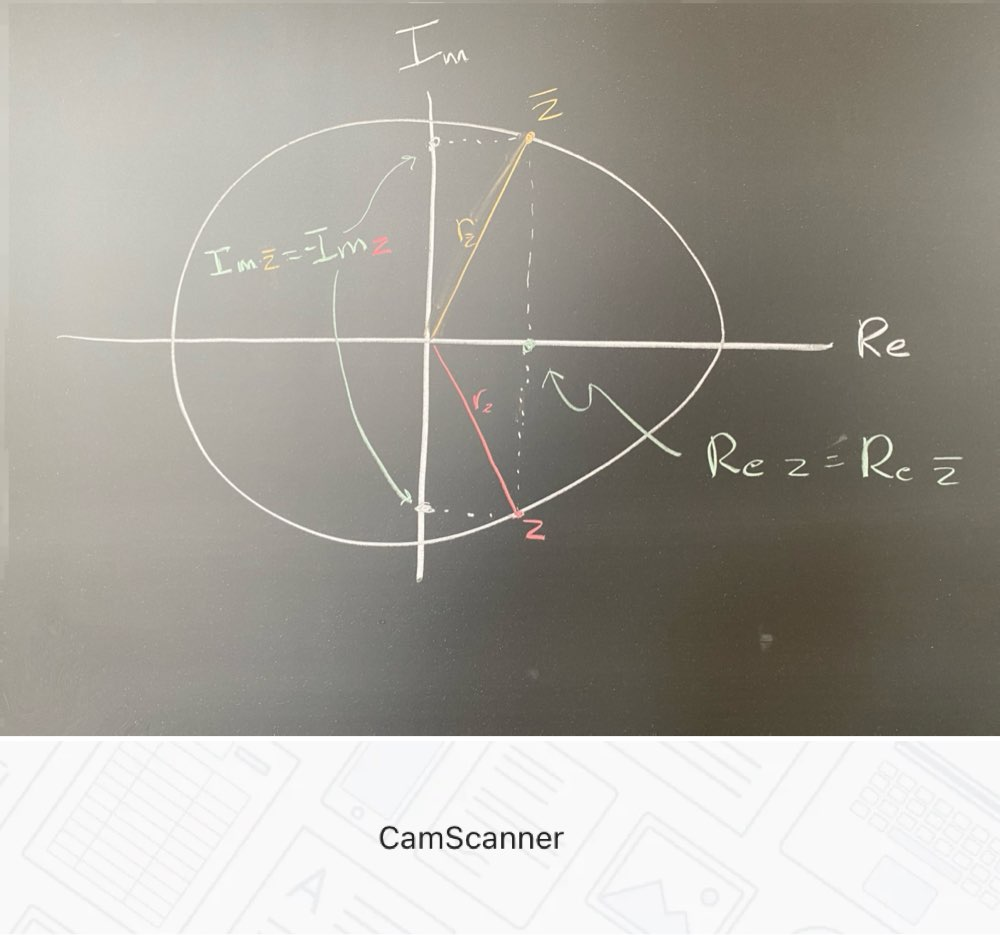
\includegraphics[width=3.5in]{Long image 2024-02-09 11.29.57.jpg}
\end{figure}
\end{itemize}

\vspace{0.1 cm}

\item[(b)] 
   \begin{itemize}
      \item[(i)] $$\frac{i^{2}}{i^{3}-4i+6}= \frac{-1}{-i-4i+6}= \frac{-1}{6-5i}\cdot \frac{6+5i}{6+5i}=\frac{-6-5i}{36-25i^{2}}= \frac{-6-5i}{61}$$so, the real part is $\frac{-6}{61}$ and the [[Imaginary Part]] is $\frac{-5}{61}$
        \vspace{0.1 cm}
      \item[(ii)]$$e^{4(2+\sqrt{2}i)t}=e^{8t}e^{4\sqrt{2}it}=e^{8t}(\cos4\sqrt{2}t+i\sin4\sqrt{2}t)$$so, the [[Real Part]] is $e^{8t}\cos 4\sqrt{2}t$ and the [[Imaginary Part]] is $e^{8t}\sin 4\sqrt{2}t$
   \end{itemize}
   
   \vspace{0.1 cm}
   
\item[(c)]
  \begin{itemize}
      \item[(i)]$$|(2-i)^{2}\cdot(4+6i)|=|2-i|^{2}|4+6i|=(4+1)\sqrt{16+36}=5\sqrt{52}$$
        \vspace{0.1 cm}
      \item[(ii)]$$\left|\left(\frac{i+2}{i-2}\right)^{57}\right|=\left(\frac{|i+2|}{|i-2|}\right)^{57}=\left(\frac{1+4}{1+4}\right)^{57}=1$$
        \vspace{0.1 cm}
      \item[(iii)]$$|(2+3i)e^{2+i}|=|2+3i||e^{2+i}|=\sqrt{4+9}e^{2}=e^{2}\sqrt{13}$$
  \end{itemize}   
\end{itemize}

\vspace{0.2 cm}

\item {\bf{Problem 4:}} 

\vspace{0.1 cm}
\begin{itemize}
\item[(a)]

Let $P(n)$ be $$\sum_{k=0}^{n}z^{k}= \frac{1-z^{n+1}}{1-z}$$

Base case: $n=0$
$$\sum_{k=0}^{0}z^{k}=z^{0}=1$$and $$\frac{1-z^{0+1}}{1-z}=\frac{1-z}{1-z}=1$$since $z\ne1$. Therefore, $P(0)$ holds.

Inductive Step: Let $n\ge0$ be given and assume $P(n)$ holds. 
Then, \begin{align*}\sum_{k=0}^{n+1}z^{k}&=\sum_{k=0}^{n}z^{k}+z^{n+1}= \frac{1-z^{n+1}}{1-z}+z^{n+1}=\frac{1-z^{n+1}+z^{n+1}(1-z)}{1-z}\\
&=\frac{1-z^{n+1}+z^{n+1}-z^{n+2}}{1-z}= \frac{1-z^{n+2}}{1-z}\end{align*}Therefore, $P(n+1)$ holds.

So by (PMI), $P(n)$ for all $n\in \mathbb{N}$.

\vspace{0.1 cm}
\item[(b)] 

Goal: $$\sum_{k=1}^{n}\sin kt=\frac{\sin \frac{1}{2}(n+1)t\cdot\sin\frac{1}{2}nt} {\sin \frac{1}{2}t}$$
Note that
$$\sin \theta=\text{Im}(e^{i\theta})$$
So, $$\sum_{k=1}^{n}\sin kt=\sum_{k=1}^{n}\text{Im}(e^{ikt})=\text{Im}\left(\sum_{k=1}^{n}e^{ikt}\right)=\text{Im}\left(\sum_{k=1}^{n}e^{ikt}+1\right)$$
and, \begin{align*}\sum_{k=1}^{n}e^{ikt}+1&=\sum_{k=0}^{n}(e^{it})^{k}= \frac{1-(e^{it})^{n+1}}{1-e^{it}}\quad(\text{by part a})\\
&=\frac{e^{it\frac{n+1}{2}}\left(e^{-it\frac{n+1}{2}}-e^{it\frac{n+1}{2}}\right)}{1-e^{it}}\\
&= \frac{e^{it\frac{n+1}{2}}\left(-2i\sin t\frac{n+1}{2}\right)}{1-e^{it}}\cdot \frac{1-e^{-it}}{1-e^{-it}}\\
&= \frac{-2i\sin t\frac{n+1}{2}(e^{it\frac{n+1}{2}}-e^{it\frac{n-1}{2}})}{1-e^{-it}-e^{it}+1}\\
&= \frac{-2i\sin t\frac{n+1}{2}(e^{it\frac{n+1}{2}}-e^{it\frac{n-1}{2}})}{2-2\cos t}\\
&= \frac{i\sin t\frac{n+1}{2}\left(e^{it\frac{n+1}{2}}-e^{it\frac{n-1}{2}}\right)}{\cos t-1}
\end{align*}
and \begin{align*}
e^{it\frac{n+1}{2}}-e^{it\frac{n-1}{2}}&= \cos t\frac{n+1}{2}+i\sin t\frac{n-1}{2}-\cos t\frac{n-1}{2}-i\sin t\frac{n-1}{2}\\
\cos t\frac{n+1}{2}-\cos t\frac{n-1}{2}&= \cos \frac{tn}{2}\cos \frac{t}{2}-\sin \frac{tn}{2}\sin \frac{t}{2}-\cos \frac{tn}{2}\cos \frac{-t}{2}\\&+\sin \frac{tn}{2}\sin \frac{-t}{2}\\
&= \cos \frac{tn}{2}\cos \frac{t}{2}-\cos \frac{tn}{2}\cos \frac{t}{2}\\
&-\sin \frac{tn}{2}\sin \frac{t}{2}-\sin \frac{tn}{2}\sin \frac{t}{2}\\
&= -2\sin \frac{tn}{2}\sin \frac{t}{2}\\
\cos t-1&= -2\sin^{2} \frac{t}{2}
\end{align*}
So, \begin{align*}\text{Im}\left(\sum_{k=1}^{n}e^{ikt}\right)&= \frac{\sin t\frac{n+1}{2}\cdot-2\sin \frac{tn}{2}\sin \frac{t}{2}}{-2\sin^{2} \frac{t}{2}}\\
&= \frac{\sin \frac{1}{2}t(n+1)\sin \frac{1}{2}tn}{\sin \frac{1}{2}t}
\end{align*}

\end{itemize}

\vspace{0.2 cm}

\item {\bf{Problem 5:}} 

\begin{itemize}
\item[(a)]


\begin{lemma}
For all $x,y\in \mathbb{R}$, $$x^{2}\le y^{2}\implies |x|\le |y|$$
\end{lemma}

\textit{Proof:}
Since $x^{2}=|x|^{2}$, 
$$0\le y^{2}-x^{2}=(|y|-|x|)(|y|+|x|)$$so, $$0\le|y|-|x|\implies |y|\ge|x|$$ 


Triangle Inequality:

$$|z+w|^{2}=(z+w)\cdot(\overline{z+w})$$
Let $z=a+ib$ and $w=c+id$. We have the following: \begin{align*}z+w&= (a+c)+i(b+d)\\
\overline{z+w}&= (a+c)-i(b+d)\end{align*}
So, \begin{align*}
|z+w|^{2}&= (a+c)^{2}-i^{2}(b+d)^{2}\\
&= a^{2}+2ac+c^{2}+b^{2}+2bd+d^{2}\\
&= a^{2}+b^{2}+c^{2}+d^{2}+2ac+2bd
\end{align*}And, \begin{align*}(|z|+|w|)^{2}&= |z|^{2}+2|z||w|+|w|^{2}\\
&= a^{2}+b^{2}+c^{2}+d^{2}+2|z||w|
\end{align*}
If $2|z||w|\ge2ac+2bd$, then we are done. \begin{align*}
|z|^{2}|w|^{2}&= (a^{2}+b^{2})(c^{2}+d^{2})\\
&= a^{2}c^{2}+a^{2}d^{2}+b^{2}c^{2}+b^{2}d^{2}\\
(ac+bd)^{2}&= a^{2}c^{2}+2acbd+b^{2}d^{2}
\end{align*}Taking the difference, the desired inequality is:
$$a^{2}d^{2}+b^{2}c^{2}\ge 2adbc$$which may be rewritten:
$$a^{2}d^{2}-2adbc+b^{2}c^{2}\ge0$$
and simplified to
$$(ad-bc)^{2}\ge0$$
This is true, since the square of any real number is nonnegative. We conclude that $$|z+w|^{2}\le(|z|+|w|)^{2}$$So by Lemma 1.1, (2.37) holds.




\vspace{0.1 cm}

\end{itemize}

\end{itemize}


\end{document}

%------------------------------------------------------------------------------
% End of journal.tex
%------------------------------------------------------------------------------
